\newlecture

\setcounter{section}{3}
%\def\textbookchapter{Chapter 9: Multivariable and Vector Functions}
\def\coursetopicnumber{I}
\def\textbooksection{9.4} % corresponding textbook section
\def\topic{The Cross Product} % this is the printed title
\def\shorttopic{Cross product} % short topic
\def\textbookname{Active Calculus} % this is the textbook
\def\textbooksectionurl{https://activecalculus.org/vector/S-9-4-Cross-Product.html} % URL for textbook section
\def\handoutday{} % this is the printed date

%%%%%%%%% DOCUMENT CONTENT STARTS BELOW

\thispagestyle{plain}
\topstuff
\section{\topic{} \booklink{}}
\label{sec:cross-product}
The cross product gives us another way to ``multiply'' one vector by another vector.

\subsection{Cross product: General definition}
\begin{framed}
    \begin{defn}
        For vectors $\vec{u}$, $\vec{v}$ in $\mathbb{R}^3$, the \emph{cross product of $\vec{u}$ and $\vec{v}$}, \\ written $\vec{u}\times\vec{v}$, is the unique vector in $\mathbb{R}^3$ that
        \begin{itemize}
            \item is orthogonal to both $\vec{u}$ and $\vec{v}$;
            \item has magnitude equal to the area of the parallelogram with sides $\vec{u}$ and $\vec{v}$; and
            \item the vectors $\vec{u}$, $\vec{v}$, $\vec{u}\times\vec{v}$ satisfy the right-hand rule.%\footnote{Image below from \url{https://commons.wikimedia.org/wiki/File:Right_hand_rule_cross_product_large_print.svg}.}.
        \end{itemize}
        In other words, for $\vec{w}=\vec{u}\times\vec{v}$, we have \\ \begin{minipage}{.6\textwidth}
            \begin{itemize}
                \item \hide{$\vec{u}\dotp\vec{w}=0$ and $\vec{v}\dotp\vec{w}=0$;}\\
                \item \hide{$|\vec{w}|$ is the area of the parallelogram formed by $\vec{u}$ and $\vec{v}$; and}\\
                \item \hide{$\vec{u}$, $\vec{v}$, $\vec{w}$ satisfies the right-hand rule (point, curl, thumb).}\\ 
            \end{itemize}
        \end{minipage}
        \hfill
        \begin{minipage}{.3\textwidth} 
            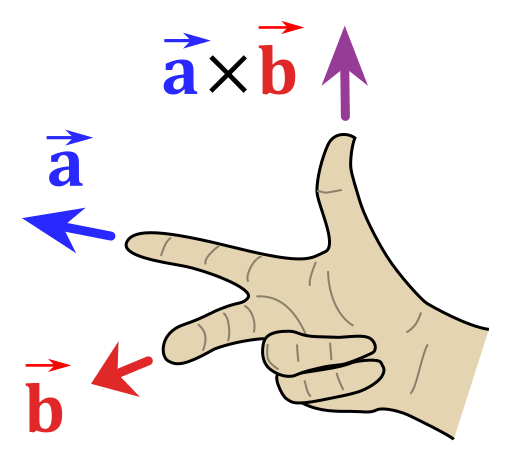
\includegraphics[width=\textwidth]{images/right hand rule cross product.png}\label{img:wikimedia-rhr-cross-product}
      \end{minipage}
    \end{defn}
\end{framed}
\noindent Note: The cross product is only defined in $\mathbb{R}^3$! It does not generalize to other dimensions. Also, some people call the cross product an \emph{external product}.

\begin{ex}
Compute the following:
	\begin{multicols}{3}
    \begin{enumerate}
    	\item $\ii \times\jj $
        \item $\jj \times\ii $
        \item $(2\kk )\times(-\jj )$
    \end{enumerate}
    \end{multicols}
\end{ex}

\vfill

\pagebreak 

\begin{ex}\label{ex:standard-unit-vec-cross-products}
    Cross products of standard unit vectors?
\end{ex}

\vspace{2in}

\begin{ex}
    How are $\vec{u}\times\vec{v}$ and $\vec{v}\times\vec{u}$ related?
\end{ex}

\vspace{2in}

\begin{ex}
    If $\vec{u}$ and $\vec{v}$ are parallel, then\bigskip
    \[\hspace{-5in}\vec{u}\times\vec{v}=\]
\end{ex}

\vspace{.5in}

\begin{ex}
    For any vector $\vec{v}$, we have $\vec{v}\times\vec{v}=$
    \bigskip
\end{ex}
\vspace{.5in}

\begin{thm}[Cross product properties]\label{thm:cross-prod-props}
    Let $\vec{u}, \vec{v}, \vec{w}$ be vectors in $\mathbb{R}^3$ and $c$ any scalar. Then
	\begin{enumerate}
    	\item $\vec{u}\times\vec{v}=\phantom{-(\vec{v}\times\vec{u})}$ \hfill{(Antisymmetry)}
    	\item $c(\vec{u}\times\vec{v})=\phantom{ 	
        (c\vec{u})\times\vec{v}=\vec{u}\times(c\vec{v})}$ \hfill{(Associativity with scalars)}
    	\item $(\vec{u}+\vec{v})\times\vec{w}=$ 
    	%\vec{u}\times\vec{w}+\vec{v}\times\vec{w}$
    	\hfill{(Distributive property)}
    	\item $\vec{u}\times(\vec{v}+\vec{w})=$ 
    	%\vec{u}\times\vec{v}+\vec{u}\times\vec{w}$
    	\hfill{(Distributive property)}
	\end{enumerate}
\end{thm}

\pagebreak 
\begin{ex}
    For $\vec{u}=3\ii +2\kk $ and $\vec{v}=-4\ii +5\jj $, use Theorem~\ref{thm:cross-prod-props} and Exercise~\ref{ex:standard-unit-vec-cross-products} to compute $\vec{u}\times\vec{v}$.
\end{ex}

\vspace{1.8in}

\begin{ex}
    Compute $(\ii +\jj )\times(\jj \times\kk )$.
\end{ex}

\vspace{.7in}

\subsection{Cross product: Geometric interpretation}
\begin{thm}
    Given two nonzero vectors $\vec{u}$ and $\vec{v}$ in $\mathbb{R}^3$, if $\theta$ is the angle between $\vec{u}$ and $\vec{v}$, then \medskip
    \[
        \hspace{-3in}|\vec{u}\times\vec{v}|=\phantom{|\vec{u}|\, |\vec{v}|\,\sin\theta,}
    \]
    \mbox{}\bigskip
    
    \noindent 
    (We'll have $0\le\theta\le\pi$.)
\end{thm}
\begin{ex}
    Suppose $\vec{u}$ and $\vec{v}$ are vectors in $\mathbb{R}^3$ that lie in the $xy$-plane. Suppose $\vec{u}$ has magnitude 3 and $\vec{v}$ has magnitude 4. For $\vec{u}$ and $\vec{v}$ originating at the origin,  if we look down at the $xy$-plane from the positive $z$-axis, we see that $\vec{u}$ points in a direction $\pi/4$ radians counterclockwise from $\vec{v}$. Compute $\vec{u}\times\vec{v}$.
\end{ex}

\pagebreak

\subsection{Interlude: Matrices and determinants}
Now we'll see a way to more efficiently compute cross products. To do so, we'll use matrices.
\begin{defn}[Matrix]
    For positive integers $m$, $n$, a \emph{matrix} is a rectangular array of numbers:
    \bigskip 

    $\displaystyle A = 
    \begin{pmatrix}
        a_{1,1} & a_{1,2} & \dots & a_{1,n} \\ 
        a_{2,1} & a_{2,2} & \dots & a_{2,n} \\ 
        \vdots & \vdots & \ddots & \vdots \\
        a_{m,1} & a_{m,2} & \dots & a_{m,n}
    \end{pmatrix}$
    \bigskip 
    
    A matrix has \emph{rows} (which are horizontal) and \emph{columns} (which are vertical). We refer to a matrix with $m$ rows and $n$ columns as an $m\times n$ (said ``$m$ by $n$'') matrix.
\end{defn}
For our work, we'll deal with determinants of $2\times2$ and $3\times3$ matrices.
\begin{defn}[Determinant]
    Suppose $A$ is a $2\times2$ matrix, so $A=\begin{pmatrix}a&b\\c&d\end{pmatrix}.$ The \emph{determinant} of $A$ is $\det(A)=\phantom{ad-bc.}\hspace{.5in}$ We can also represent this with vertical bars on the matrix:
    \begin{framed}
        \[
            \hspace{-4in}\det(A)=\phantom{|A|=\begin{vmatrix}a&b\\c&d\end{vmatrix}=ad-bc.}
        \]
    \end{framed}
\end{defn}
\begin{ex}
    If $A=\begin{pmatrix}1&4\\-3&-5 \end{pmatrix}$, compute $|A|$.
\end{ex}

\vspace{.5in}

\begin{defn}[Cofactor expansion for determinant]
    Suppose $A$ is a $3\times3$ matrix. %, so $A=\begin{pmatrix}a&b&c\\d&e&f\\g&h&i\end{pmatrix}.$ 
    The \emph{determinant} of $A$ is computed via the following \emph{cofactor expansion}:  
    
    \bigskip
    
    \noindent $\displaystyle
    \det(A) = 
    \begin{vmatrix}a&b&c\\d&e&f\\g&h&i\end{vmatrix}
    =
    \phantom{
        a\begin{vmatrix}e&f\\h&i\end{vmatrix}
        -b\begin{vmatrix}d&f\\g&i\end{vmatrix}
        +c\begin{vmatrix}d&e\\g&h\end{vmatrix}.
    }
    $
\end{defn}
\begin{ex}
    Let $A=\begin{pmatrix}
        2&3&4\\ 
        0&-5&1\\
        -3&2&10
    \end{pmatrix}$.
    Compute $|A|$.
\end{ex}
\pagebreak

\subsection{Cross product: Computational shortcut}
\begin{thm}
    Suppose $\vec{u}=\langle u_1,u_2,u_3\rangle$ and $\vec{v}=\langle v_1,v_2,v_3\rangle$. The  \emph{cross product} of $\vec{u}$ and $\vec{v}$ is 
    \begin{framed}
        \[
            \hspace{-3in}\vec{u}\times \vec{v}=\langle u_1,u_2,u_3\rangle \times \langle v_1,v_2,v_3\rangle = \phantom{\begin{vmatrix}\ii &\jj &\kk \\u_1&u_2&u_3\\v_1&v_2&v_3\end{vmatrix}.}
        \]
    \end{framed}
\end{thm}
\begin{ex}
    Expand $\vec{u}\times\vec{v}$ in terms of $2\times2$ determinants, then multiply it out.
\end{ex}

\vspace{1.3in}

\begin{ex}
Let $\vec{u}=\langle 3,0,2\rangle$ and $\vec{v}=\langle -4,5,0\rangle$.
	\begin{enumerate}
        \item Compute $\vec{u}\times\vec{v}$ using the rule above.
    	\item What is the area of the parallelogram formed by $\vec{u}$ and $\vec{v}$?
        \item What is the area of the triangle formed by $\vec{u}$ and $\vec{v}$?
    	\item Find two unit vectors that are orthogonal to both $\vec{u}$ and $\vec{v}$.
	\end{enumerate}
\end{ex}

\pagebreak 

\subsection{Applications: Area and volume}
A \emph{parallelogram} is a quadrilateral in the plane for which opposite sides are parallel. We can think of a parallelogram is being constructed by two vectors that start at the same point.

\vspace{1in}

The area of such a parallelogram is 
\bigskip

If all of the angles within the parallelogram are right angles, we call it a rectangle. The 3D analogue of a rectangle is a rectangular box. And the 3D analogue of a parallelogram is a parallelopiped!

A \emph{parallelopiped} is a 3D figure made up of 6 faces, each of which is a parallelogram. Opposite faces are parallel. We can think of a parallelopiped as being constructed by three vectors that start at the same point.

\vspace{1.7in}

\begin{thm}
    The volume of a parallelopiped constructed from vectors $\vec{u}$, $\vec{v}$, $\vec{w}$ is
    \[
        |(\vec{u}\times\vec{v})\dotp\vec{w}|.
    \]
\end{thm}
Note: The quantity $(\vec{u}\times\vec{v})\dotp\vec{w}$ is called a \emph{triple scalar product} of $\vec{u}$, $\vec{v}$, and $\vec{w}$.

\begin{ex}
    Find the volume of the parallelopiped formed by the vectors $\vec{u}=\langle 3, 5, -1\rangle$, $\vec{v}=\langle 2, -2, 1\rangle$, and $\vec{w}=\langle 3, 3, 1\rangle$.
\end{ex}
